% TEMPLATE for Usenix papers, specifically to meet requirements of
%  USENIX '05
% originally a template for producing IEEE-format articles using LaTeX.
%   written by Matthew Ward, CS Department, Worcester Polytechnic Institute.
% adapted by David Beazley for his excellent SWIG paper in Proceedings,
%   Tcl 96
% turned into a smartass generic template by De Clarke, with thanks to
%   both the above pioneers
% use at your own risk.  Complaints to /dev/null.
% make it two column with no page numbering, default is 10 point

% Munged by Fred Douglis <douglis@research.att.com> 10/97 to separate
% the .sty file from the LaTeX source template, so that people can
% more easily include the .sty file into an existing document.  Also
% changed to more closely follow the style guidelines as represented
% by the Word sample file. 

% Note that since 2010, USENIX does not require endnotes. If you want
% foot of page notes, don't include the endnotes package in the 
% usepackage command, below.

\documentclass[letterpaper,twocolumn,10pt]{article}
\usepackage{usenix, epsfig,endnotes}
\usepackage{amsmath}
\usepackage{hyphenat}
\usepackage{hyperref}
\usepackage{titlesec}
\usepackage{lipsum}
\usepackage{array}
\usepackage{alltt}

% Wrap and centering multicolumn
\newcolumntype{C}[1]{>{\centering\arraybackslash}m{#1}}

% Change caption settings
\usepackage[font=footnotesize,labelfont=bf]{caption}

% Change font and spacing
\titleformat*{\subsection}{\normalsize\bfseries}
\titlespacing{\subsection}{0pt}{0.8em}{0.8em}
\titleformat*{\subsubsection}{\small\bfseries}

% Paragraph margin
\setlength{\parskip}{0.2em}

\let\OLDthebibliography\thebibliography
\renewcommand\thebibliography[1]{
  \OLDthebibliography{#1}
  \fontsize{8pt}{10pt}\selectfont
  \setlength{\parskip}{0.2em}
  \setlength{\itemsep}{0pt plus 0.3ex}
}


\begin{document}
\fontsize{9pt}{11pt}\selectfont
\hyphenation{DevOps mccabe}
%don't want date printed
\date{}

%make title bold and 14 pt font (Latex default is non-bold, 16 pt)
\title{\LARGE \bf Python and Parallel Programming}

\author{
\rm{Shichao An}\\
\rm \small New York University\\
\rm \small {shichao.an@nyu.edu}
}

\maketitle

% Use the following at camera-ready time to suppress page numbers.
% Comment it out when you first submit the paper for review.
%\thispagestyle{empty}


\subsection*{Abstract}
This paper studies how to utilize parallelism in Python applications by comparing three different parallel programming methods. CPython's multithreading interface \verb#threading# and process-based ``threading'' interface \verb#multiprocessing# are discussed in terms of employing built-in functionalities, and OpenMP through \verb#cython.parallel# in Cython are introduced in terms of thread-based native parallelism.

CPU-bound and I/O-bound programs are parallelized using these methods to demonstrate features and to compare performances. As essential supplements, a derivative CPU-bound application and a matrix multiplication program are parallelized to study the overhead and memory aspect.

\section{Introduction}
The difficulty involved with writing and debugging parallel code has become one obvious obstacle to developing parallel programs. With the development effort being the bottleneck and the prevalence of multiprocessor and multicore systems, it is a rational approach to give priority to efficient development and testing techniques and reusable parallel libraries rather than machine efficiency \cite{hinsen}. This led to the increasing use of high-level languages such as Python, which supports multiprocessing and multithreading, and guarantees highly efficient development.

The standard library of Python's reference implementation, CPython (2.x), provides the following built-in modules: the lower-level \verb#thread#, the higher level \verb#threading# and \verb#multiprocessing# module. The \verb#threading# module provides an easy-to-use threading API built on top of the \verb#thread# module, and the \verb#multiprocessing# module applies a similar interface to spawning and managing subprocesses.

Most programmers will intuitively starts with the default multithreading module, \verb#threading#. It makes use of real system threads and provides friendly thread management interface and synchronization mechanisms such as Lock, RLock, Condition and Semaphore. However, the Global Interpreter Lock ensures that only one thread can execute Python code at once. This makes it easier for the interpreter to be multi-threaded, but is at the expense of much of the parallelism afforded by multicore and multiprocessor machines \cite{glossary}.

When realizing the restrictions of GIL and requiring to make better use of the computational resources, programmers may choose \verb#multiprocessing# to side-step GIL. It gives a similar interface to \verb#threading# but uses subprocesses to enable the programmers to fully leverage multiple processors. However, it also brings overhead in process switching and inter-process communication. 

Given the nature of GIL and the expense of multiprocessing, native parallelism should be considered while still keeping an eye on development efficiency. Cython with OpenMP is such a solution that seems less intuitive but appeals to those familiar with OpenMP. It makes it easier to integrate with existing Python code and releases GIL for better parallel performance.

This paper provides a comprehensive study of the three approaches by comparing them under different circumstances and analyzing features in regard to the comparison of the performances. It aims at providing an evaluation report to help programmers better decide the programming method to efficiently parallelize their various applications.

\section{Literature Survey}
Use of Python on shared-memory multiprocessor or multicore systems is prevalent. Much of the work employs Python in scientific computing field, e.g. parallel numerical computations. Other work discusses specific aspects in a more general field.

Masini et al. \cite{masini} present the porting process of a multicore eigensolver to Python and discuss the pros and cons of using Python in a high-performance parallel library. They focus on Python's advantages in improving code readability, flexibility and correctness compared to C and Fortran within parallel numerical computations. The work also introduces performance issues by explaining impact of the Global Interpreter Lock. However, their work does not discuss in detail the multithreading in terms of parallelism, and fails to give an alternative or solution to the performance overhead and contention.

The parallelization experiments using \verb#multiprocessing# and \verb#threading# by Eli Bendersky \cite{bendersky} reveals more relevance to my work. The demonstration of parallelizing CPU-bound tasks has greatly influenced my thinking. It gives a complete benchmark of the serial, multithreading, and multiprocessing programs to demonstrate Python thread's weakness in speeding up CPU-bound computations and the simplicity of parallelizing code using \verb#multiprocessing#. Another experiment in \verb#threading# also mentions the applicable scope of Python thread. However, these experiments have not presented an comparison of multithreading and multiprocessing in parallelizing I/O bound and memory-bound programs to make a thorough conclusion.

David Beazley's \cite{dabeaz1}\cite{dabeaz2} articles and presentations provide elaborate illustrations of Global Interpreter Lock (GIL) with exploration from Python script to C source code. His work delves into the behind-the-scenes details of GIL by analyzing behavior and implementations from both the interpreter and operating system perspectives. While many aspects in his work are far beyond the scope of this paper, his focus is on GIL's impact on Python thread in doing CPU-bound and I/O-bound tasks. The study is essentially about the threading behavior and potential improvement of the GIL itself, not the more general approach of parallel programming in Python. 

In other related work \cite{rudd}\cite{molden}, the implementations simply adopt either of threading or multiprocessing without comparing the two and generalizing pros and cons. They don't discuss under what circumstances one method is applicable. My work provides an overview that encapsulates different parallel programming approaches by discussing the advantage and drawback of each and reckoning their applicable scopes as result of parallelizing CPU-bound, I/O-bound and memory-bound programs.

\section{Proposed Idea}

Despite the fact that \verb#threading#, \verb#multiprocessing# and Cython/OpenMP address parallel problems at different levels of granularity, they are still often used as alternatives to each other, especially when the drawbacks of one becomes the bottleneck under a specific circumstance. This is largely due to their implementation discrepancies, which may in return bring improvement of either performance or development efficiency. In order to demonstrate various aspects of the three approaches, several sample programs are chosen and parallelized using these approaches. The concentration is on the parallelization of the CPU-bound and I/O-bound programs, and parallelization of the memory-bound program and the overhead analysis focuses on comparing the efficiency of different types of supported data structures and performance loss of multi-threaded and multi-processing programs.

Parallelizing Python programs does not have much difference from parallelizing programs in other languages. It is a common approach to identify parallelism, enforce dependencies and handle synchronization. The essential part is to think of the problem in terms of a Python programmer who wants things done in the most ``intuitive way''. This means it is better to use the simplest supported interfaces (packages, modules, functions and data structures) that is clearly understandable with least coding and debugging effort while ensuring correctness. 

When implementing a parallel version using one approach, comparable counterparts of other approaches should be taken into account. For example, when implementing a global list with the \verb#threading# approach, the correspondingly applicable data structures  in \verb#multiprocessing# approach such as Array in shared memory or ListProxy should be considered instead of using other data structures such as \verb#Queue# with a different implementing logic, unless the entire parallel pattern is otherwise different. Keeping the similarity of logic in this way gives programmers a better observation on the performance.

However, the above rule has a disadvantage that may cause loss in performance when implementing other approaches. In Cython, for instance, the global interpreter lock (GIL) cannot be released if manipulating Python built-ins or objects in parallel sections, which makes it impossible to achieve native parallelism. Therefore, a better solution is to find a balance that deals with both aspects and put the analysis of annoying factors into an independent experiment. As a promising result, further parallelization can be performed to demonstrate the side-effects compared to the serial version, such as GIL restrictions, overhead in managing threads or processes, and contentions in using locks, which will be included in the overhead analysis programs.

With the abovementioned parallelization work done, comparison of the parallelized programs makes more sense, particularly in two major criteria: development efficiency and performance. The complexity of the parallelized program, which may be reflected by many factors such as total number of lines of code, determines the primary development effort. The compatibility is also one aspect that programmers pay much attention to in order to interface with existing applications. This generally involves the conversion of data structures under these approaches. Unlike scripting, Cython/OpenMP requires extra setup script and compile procedure that is platform-dependent, which also affects development efficiency with increased DevOps workload and portability impact.

Besides development, the performance is important in most cases and is obtained by benchmarking. It provides basis on which the overhead, produced by various factors such as thread/process creation and scheduling, the GIL and data structures, can be analyzed. By comparing the performances of the implementation of these approaches, the overall applicability of each approach can be determined, which comprises the ultimate goal of this paper. 

\section{Experimental Setup}
\subsection{Environment}
The experiments will be conducted on a MacBook Pro with an Intel Core i7 (2.9 GHz, 4 MB on-chip L3 cache, 2 physical cores, 4 logical cores \cite{core}). The operating system is OS X 10.8.5 (Darwin 12.5.0, x86\_64). The applications and their parallelized versions are programmed in Python 2.7.3 and Cython 0.19.2 under virtualenv 1.9.1. The GCC version is 4.2.1 (Apple Inc. build 5666), which supports the OpenMP v2.5 specification.


\subsection{Experimental Applications}
There are four groups of applications under study in the experiments. Each group has an original sequential program labeled as \textit{serial} and its parallelized versions using \verb#threading#, \verb#multiprocessing#, and Cython/OpenMP approaches, which are labeled as \textit{mt}, \textit{mp}, and \textit{omp} respectively. The following paragraphs in this subsection gives descriptions of each application group as for what tasks they are doing. The parallelization procedure will be discussed in the \textbf{Experiments and Discussion} section.

 \textbf{CPU-bound}. This application performs a time-consuming task that processes a freshly generated file of data. The file contains lines of origin, destination and in-between distance that are represented in random integers. The task is to remove the duplicate appearances of origin and destination and fix the distance of those lines where origin and destination are reversed to generate a consistent list. The program is expected to be CPU-bound which can be ensured using \verb#psutil# (discussed in the next subsection).
  
 \textbf{I/O-bound}. This application is a simple word parser that checks whether each possible combinations of words in the input sentence or paragraph comprises an accessible title of article on Wikipedia. It performs a large amount of successive HTTP GET requests to the Wikipedia API to analyze the returned JSON responses and generates the output which lists all titles of the accessible entries.
  
 \textbf{Memory-bound}. This is a trivial matrix multiplication program that manipulates large matrices, where two random matrices are multiplied. Although in practice this program is not necessarily memory-bound (otherwise must be CPU-bound), it is assumed to be memory-bound due to the nature of matrix-vector multiplication. With simplicity in the source code, this program is also applicable to the illustration of statically and dynamically typed comparison in Python and Cython.
  
 \textbf{Overhead analysis}. This one is derived from the CPU-bound program but does a different task. It processes the output from the CPU-bound program and performs calculations. After that, it outputs the maximum and minimum distances in that list as well as a list of origin and destination, each with the smallest in-between distance. As the task is not time-consuming, the parallelism in general will not gain any speedup but brings overhead. The parallelized programs can illustrate the overhead generated in the thread/process management and from using different data structures supported in \verb#multiprocessing#.

\subsection{Profilers and Benchmarks}
In the experiments, the following tools will be used to profile and benchmark programs after parallelization.


The \verb#time# function of Python's \verb#time# module will be used for timing programs (real time). The programs are non-trivial, so it is better to measure the wall-clock time to reflect the production environment. This is the primary benchmark that comprises most of the evaluation results.

To further measure user and system times of the processes for analysis purpose, \verb#psutil# will be used as a general process status utility in a programmatic way \cite{psutil}. It can also be used to help determine the types of programs by checking CPU usage and network connections. \verb#cProfile#, the standard profiler for Python, will be used to provide deterministic profiling for the programs to find bottlenecks.

As one of the major comparison criterion in the parallelization experiments, development efficiency needs manual evaluation from a different analysis perspective from that of performance. This means some subjectiveness may be included, such as programming effort to ensure interface compatibility and debugging difficulty (such as Cython's compile time check). However, code checking tools such as \textit{flake8} \cite{flake8} and \textit{CLOC} \cite{cloc} will still be used to help measure development efficiency by providing substantial statistics like McCabe complexity (cyclomatic complexity) and lines of code.


\section{Experiments and Discussion}
The development efficiency and performance are two major measures to make an evaluation overview of the parallelizing methods. 

Development efficiency is evaluated by comparing the parallelized source code with the original sequential one and measuring specific criteria as follows:

\vspace{-0.5em}
\begin{itemize}
\setlength{\itemsep}{-0.3em}
  \item Number of additional necessary interfaces used to perform parallelization and to ensure correctness (thread-safe);
  \item Effort to ensure interface compatibility with the original program;
  \item Extra configuration and debugging steps for the parallelized program; 
  \item Increment in the program complexity.
\end{itemize}
\vspace{-0.5em}

Performance is evaluated from the timing perspective with the following criteria:

\vspace{-0.5em}
\begin{itemize}
\setlength{\itemsep}{-0.3em}
  \item Real time to run the parallelized programs, which reflects how much speedup or overhead it has actually brought;
  \item User/system timing of the parallelized programs, which reflects how much actual parallelism is brought;
\end{itemize}
\vspace{-0.5em}

The expected results are case dependent but can be generalized. In development efficiency, \verb#threading# should always have less coding effort and better compatibility than the other two, while Cython/OpenMP requires the most effort and thus provides least efficiency. In performance, \verb#multiprocessing# and Cython/OpenMP generally performs better than \verb#threading# in CPU intensive tasks, but \verb#threading# and Cython/OpenMP performs better in I/O-bound programs. In terms of parallelism, however, only Cython/OpenMP and \verb#multiprocessing# will bring native parallelism, while \verb#threading# cannot due to the restriction of GIL.

\subsection{Parallelization}
The parallelization is done by using each approach to implement the parallel part in each application group. This parallel part is derived from a function in the sequential program that basically works as an modularized interface. In the source code, this function is \verb#proc()# (abbreviation of \textit{processing}), which executes the parallel tasks by processing the common input and generating output, both of which are usually globally defined. As few lines of code as possible will be used in the implementation to keep a simplest logic to ensure interface compatibility and correctness.

To create multiple threads, the \verb#threading# programs always employ \verb#Thread# by specifying the \textit{target} and \textit{args} arguments with a worker function and its parameters respectively, without declaring the \verb#Thread# class. Nearly all types of data structures in this approach will be the same to those in the sequential program, which involves Python built-ins such as list and dictionary. \verb#Queue.Queue# will be used to implement multi-consumer queue for the I/O-bound programs that adopts the thread pool pattern.

The \verb#multiprocessing# approach follows the similar process creation method to \verb#threading#. It involves many shared-memory data structures that are ready-to-use Python built-in objects, such as \verb#Value#, \verb#Array# and other types of supported by the \verb#Manager# object.
In the I/O-bound parallelization, the \verb#multiprocessing.Queue()# is the counterpart of \verb#Queue.Queue# in the \verb#threading# approach.

The Cython/OpenMP approach...

The I/O-bound... The CPU-bound and overhead...

Similar pattern for observation. All approaches divide tasks into chunks (cpu-bound, memory-bound, overhead), or use thread pool pattern (io-bound)

\subsection{Results and Analysis}
\subsubsection{Performance}

The performance of each approach is evaluated against all programs parallelized. Firstly, the evaluation is conducted by measuring real times consumed by the \textit{proc()} functions, which is illustrated in Figure 1-6. In these figures, the abbreviated notation in the legend has the following meanings:

\vspace{-0.5em}
\begin{description}
\setlength{\itemsep}{0em}
  \item[\it serial:] original sequential program 
  \item[\it mt:] parallelized version using \verb#threading# approach
  \item[\it mp:] parallelized version using \verb#multiprocessing# approach with default shared-memory data types
  \item[\it mp (manager):] \raggedright parallelized version using \verb#multiprocessing# approach with data types supported by \verb#Manager#
  \item[\it omp:] parallelized version using Cython/OpenMP approach
  \item[\it omp (GIL):] without releasing the global interpreter lock (GIL)
  \item[\it omp (no GIL):] releasing the global interpreter lock (GIL)
  \item[\it omp (static type):] using C/C++ data types
  \item[\it omp (dynamic type):] using Python data types
\end{description}
\vspace{-0.5em}

\begin{figure}[h!]

  \centering
    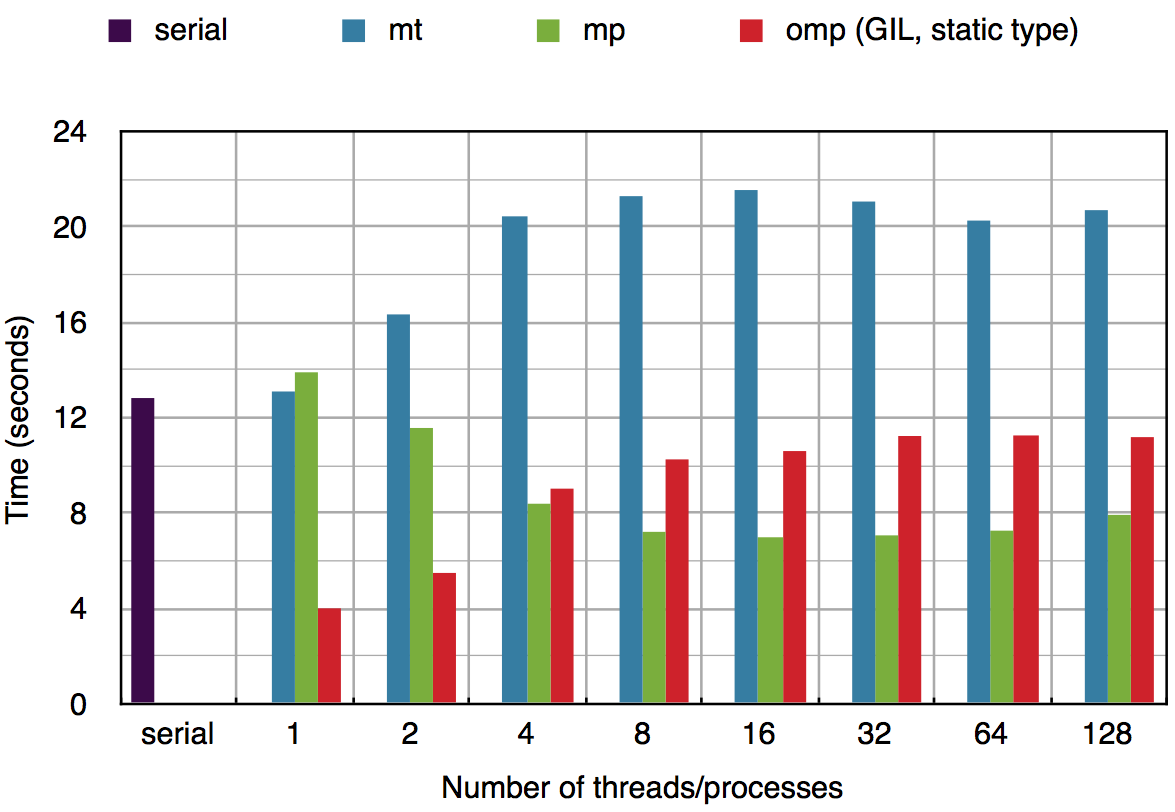
\includegraphics[width=24em]{../img/cpu_bound.png}
      \caption{CPU-bound}
\end{figure}

\begin{figure*}[t]
\centering

\begin{alltt}
\setlength{\parindent}{4em}
\small
ncalls  tottime  percall  cumtime  percall filename:lineno(function)
  768   16.755    0.022   16.755    0.022 {method 'acquire' of 'thread.lock' objects}
  128    3.805    0.030   21.515    0.168 threading.py:484(start)
  128    0.941    0.007   16.305    0.127 threading.py:234(wait)
  128    0.011    0.000    0.011    0.000 {thread.start_new_thread}
  256    0.010    0.000    0.010    0.000 threading.py:185(__init__)
\end{alltt}
 \caption{cProfile result of \textit{mt} approach in the CPU-bound application group}
\end{figure*}


In the evaluation of CPU-bound application group (Figure 1), the behaviors of the approaches is diversified. The \textit{mt} approach is sensitive to the number of threads ($n$) and produces much overhead as $n$ increases exponentially.  Figure 2 shows the profile results of the  \textit{mt} approach, ordered by \textit{tottime}, which is the total time spent in the given function (and excluding time made in calls to sub-functions). Significant time is spent on \textit{acquire} method of \textit{thread.lock} objects, which is a major cause of the overhead generated during thread switching. This is essentially due to the fact the GIL ensures that only one thread runs in the Python interpreter at once and only the thread that has acquired the GIL may operate on Python objects or call Python/C API function \cite{gil}. The $mp$ approach performs better as $n$ increases because the subprocesses can run simultaneously without being restricted by the GIL. Though overhead is produced especially when $n$ is large, parallelism predominates so that the speedup is obvious. 

The \textit{omp (no GIL)} approach of the CPU-bound group behaves somewhat opposite to \textit{mp}. The true parallelism does not bring speedup as it cannot efficiently access the \textit{tg} array, which is a memoryview \cite{mv}  on the NumPy array \textit{ntg} (\textit{target\_list}), when multi-threaded (this is the case in this program only, and may not apply to all CPU-bound programs). As seen in Table 1, when $n$ (number of threads) is 8, the total \textit{user time} of \textit{cpu\_bound.omp (no GIL, static type)} is around 39 seconds, which indicates the average \textit{user time} of each thread is around 5. This is even larger than that of the single-threaded \textit{omp (no GIL)} version. The \textit{omp (GIL)} approach, however, makes OpenMP aware of the GIL which wraps all code region within the parallel for loop. This essentially limits the parallelism of OpenMP and it always behaves like single-threaded whatever $n$ is. Both \textit{omp (no GIL)} and \textit{omp (GIL)} operates on statically typed data, so approximate three-times speedup were gained.

\begin{figure}[h!]

  \centering
    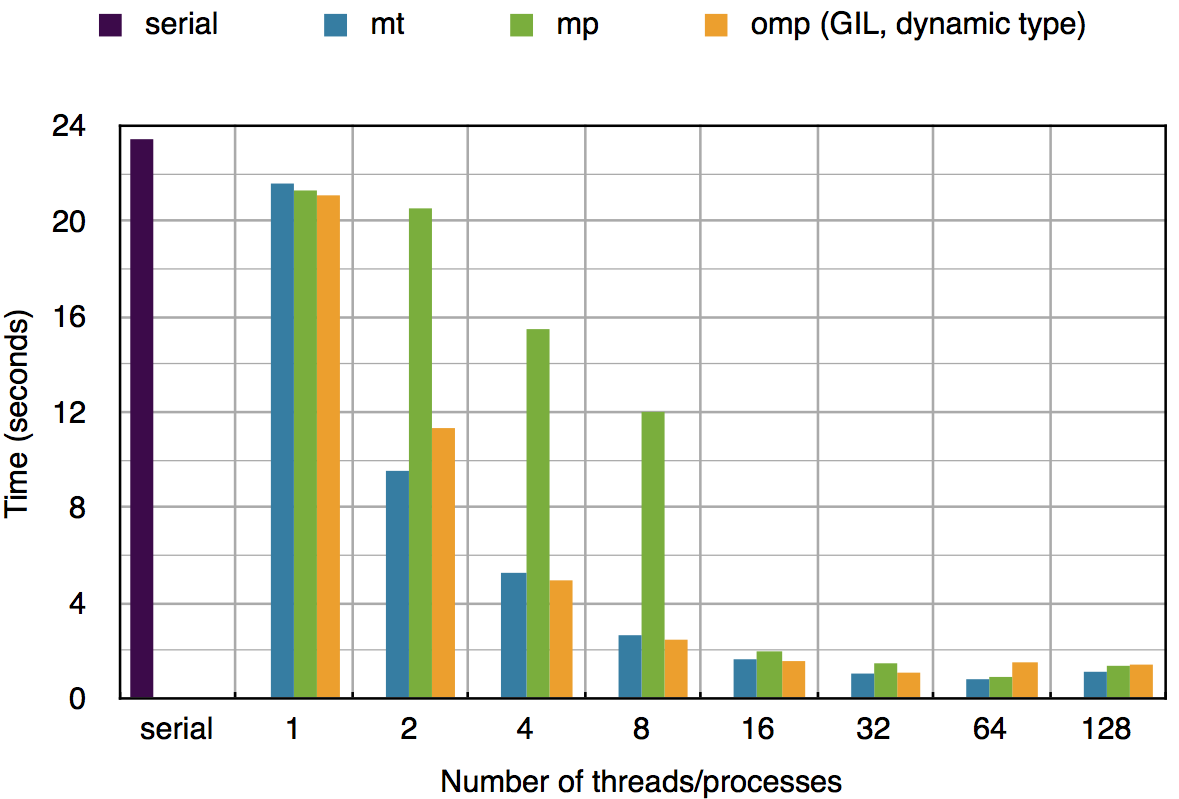
\includegraphics[width=24em]{../img/io_bound.png}
      \caption{I/O-bound}
\end{figure}

In the I/O-bound application group (Figure 2), \textit{mt} and \textit{omp (GIL, dynamic)} approaches share similar behaviors. For \textit{mt}, when the threads are doing I/O, the GIL is always released \cite{glossary}. Another behavior shows \textit{mp} does not gain much speedup when $n$ is below 8 but gains relatively same speedup as \textit{mt} and \textit{omp (GIL, dynamic)} when $n$ is larger. Through observation, it is found that the subprocesses usually cannot finish their divided chunks of tasks in fairly equal time. Due to the process scheduling, some processes may take extraordinarily longer time to join than the other processes, which becomes the bottleneck. However, when $n$ is larger, each chunk of task is relatively smaller and each process can finish the task in short time before being preempted by the process scheduler.

\begin{figure}[h!]
  \centering
    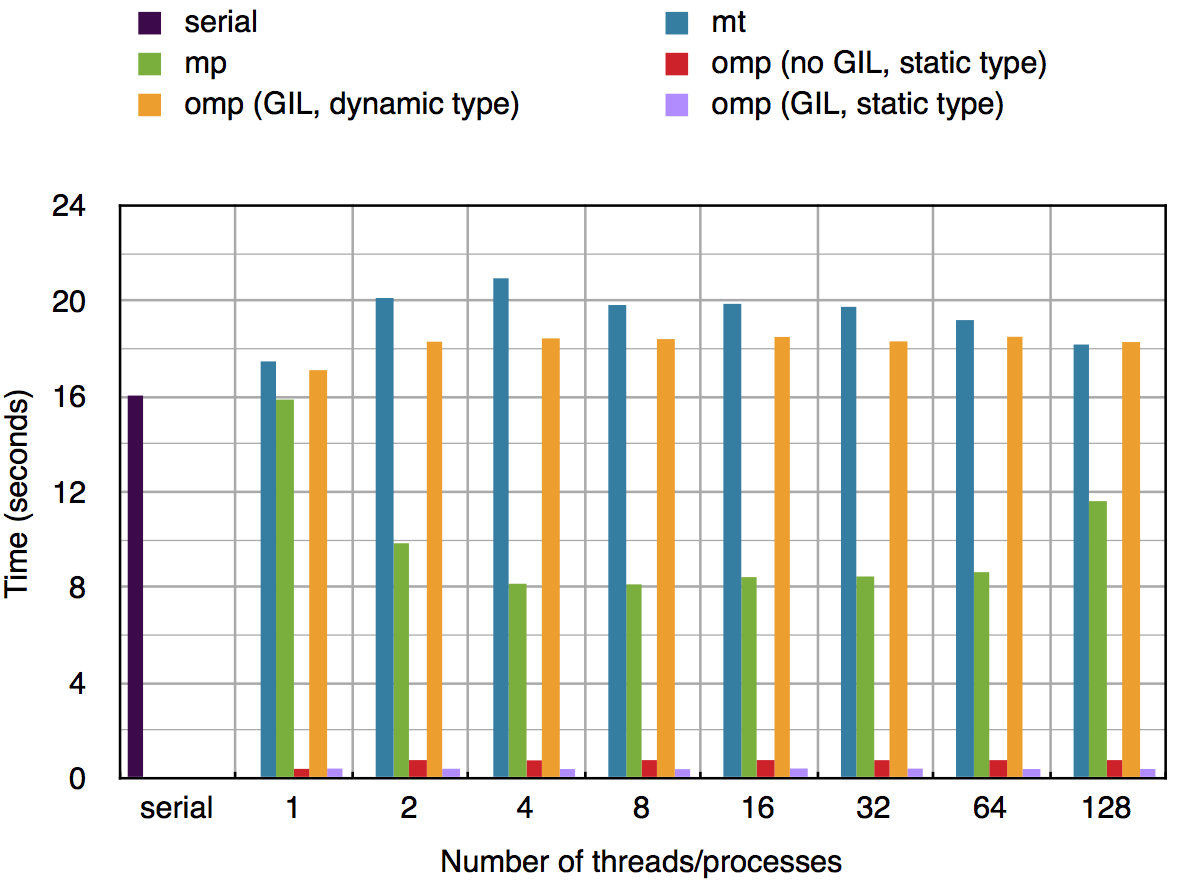
\includegraphics[width=24em]{../img/memory_bound_1.png}
      \caption{Memory-bound (1)}
\end{figure}

\begin{figure}[h!]
  \centering
    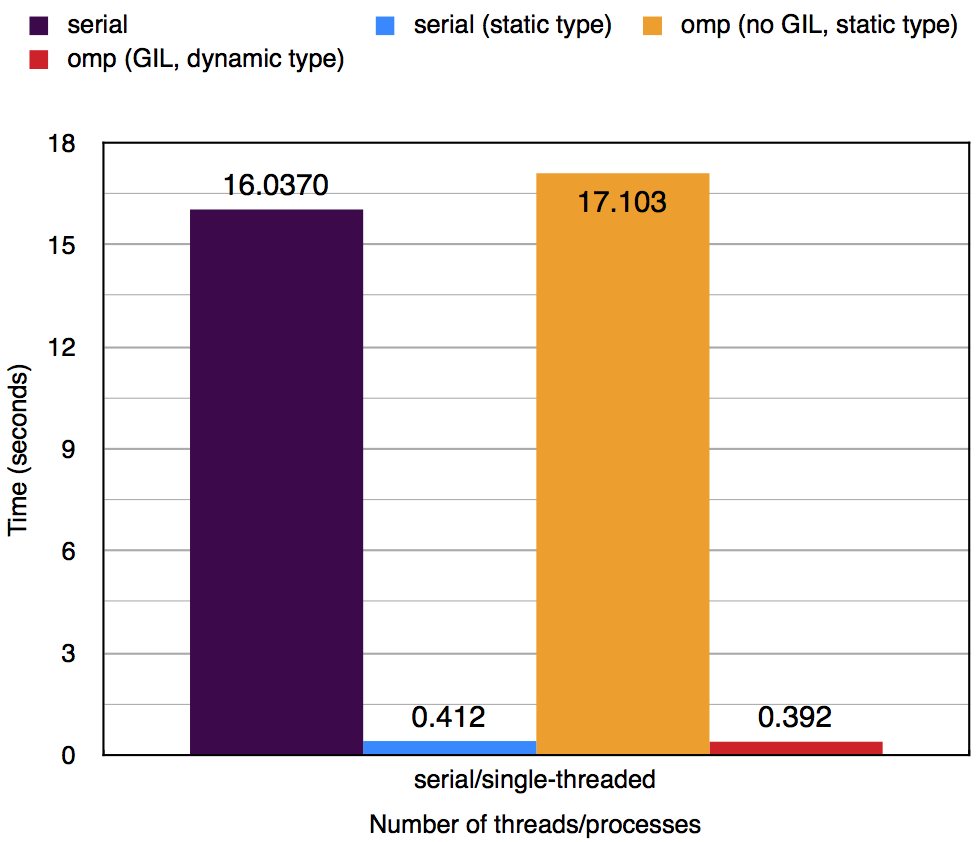
\includegraphics[width=24em]{../img/memory_bound_2.png}
      \caption{Memory-bound (2)}
\end{figure}

The behaviors of \textit{mt} and \textit{mp} in the memory-bound application group (Figure 3) can be explained similarly to those in the CPU-bound. When single-threaded, the \textit{omp (no GIL, static type)} and \textit{omp (GIL, static type)} are also similar; the former suffers from overhead when multithreaded. The efficient memory access of the matrices in these two approaches, which is a statically typed memoryview on a 2D NumPy array, brings predominant performance boost. The \textit{omp (GIL, dynamic type)} approach is rather like a counterexample that behaves similarly to \textit{mt}. To further demonstrate the performance gap between two types of data, Figure 4 is made to specifically compare \textit{serial} (sequential) and \textit{omp} approaches with different types.

\begin{figure}[h!]
  \centering
    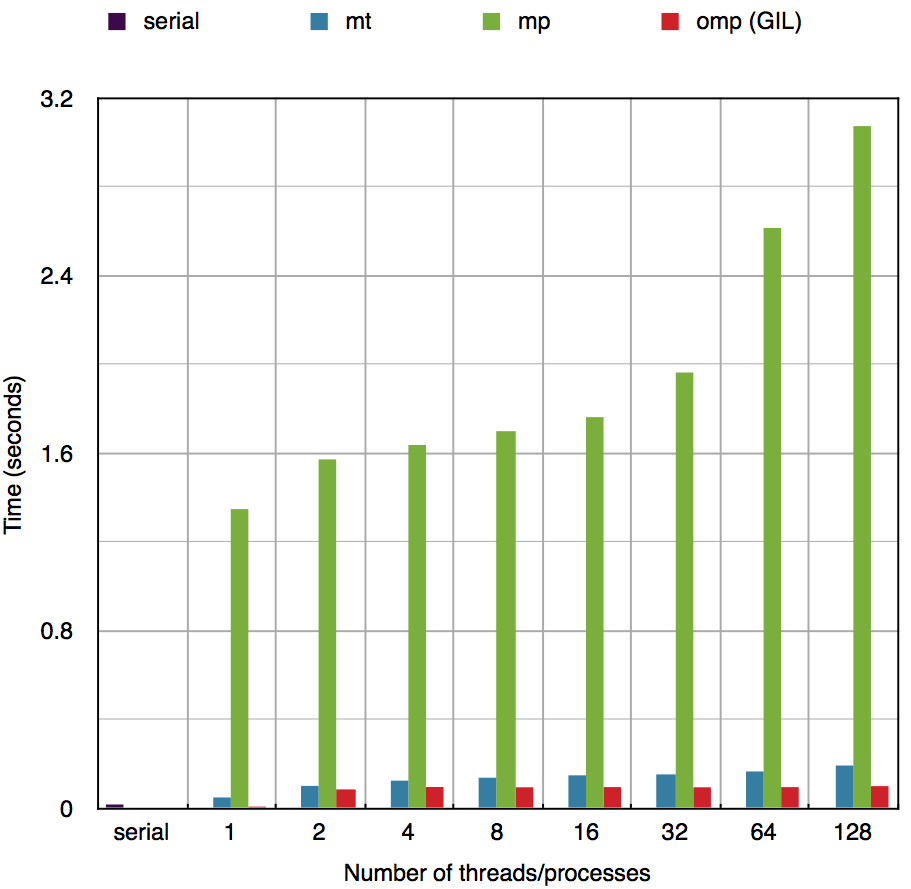
\includegraphics[width=24em]{../img/overhead_1.png}
      \caption{Overhead analysis (1)}
\end{figure}

\begin{figure}[h!]
  \centering
    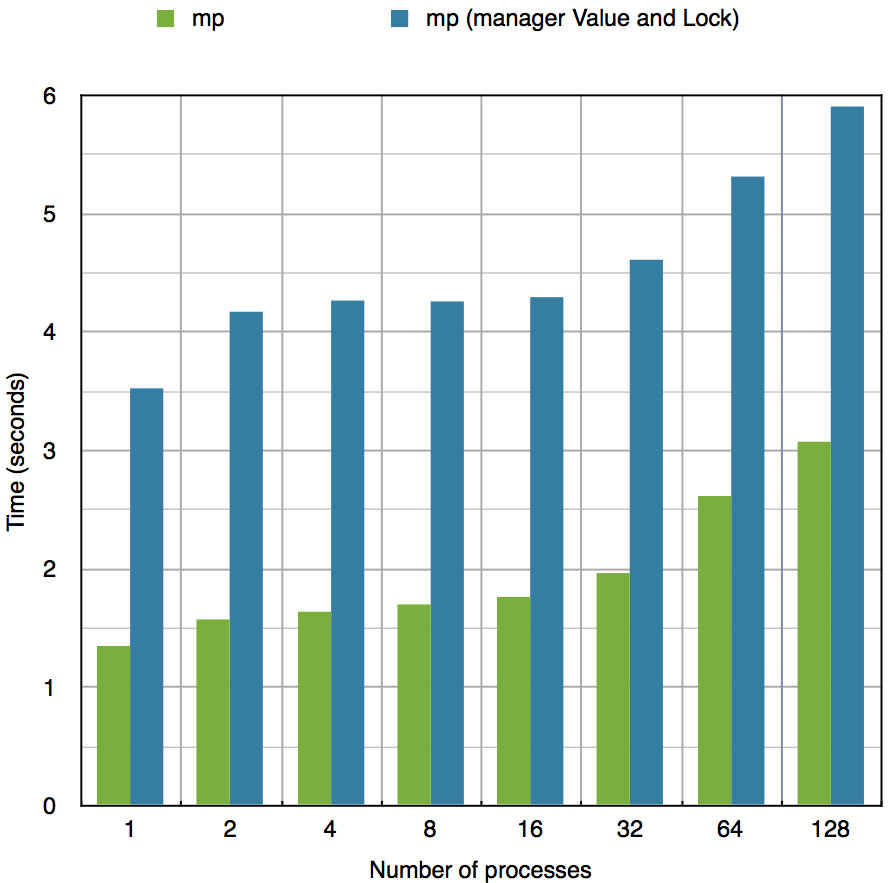
\includegraphics[width=24em]{../img/overhead_2.png}
      \caption{Overhead analysis (2)}
\end{figure}

The overhead analysis group (Figure 6 and 7) focuses on the circumstances where overhead is predominant. Particularly for \textit{mp} approach, most of the overhead originates from using the shared memory data and locks supported by the \verb#multiprocessing# module. In Figure 7, another comparison between efficiency gap between shared memory and manager implementations of the $mp$ approach. A manager object returned by \verb#Manager()# controls a server process which support arbitrary object types and allows other processes to manipulate them using proxies. It is slower than the shared memory, but can be shared by processes on different computers over a network. \cite{sp} 

Table 1 lists the times for all approaches under the measured application groups. The predominant user times are highlighted. The \textit{cpu\_bound.mp}, \textit{memory\_bound.mp} and \textit{cpu\_bound.omp (no GIL, static type)} lines reveal native parallelism that \verb#multiprocessing# and Cython/OpenMP are able to make. In these lines, the user times are approximately four times the real times, which generally reflects the number of logical cores on the testing machine.

\begin{table*}[t]
\centering
\footnotesize
\begin{tabular}{|l|r|r|r|r|r|r|}
\hline 
\multicolumn{1}{|C{5em}|}{\bf Program} &
\multicolumn{1}{C{5em}|}{\bf Proc time} &
\multicolumn{1}{C{5em}|}{\bf Real time} &
\multicolumn{1}{C{5em}|}{\bf User time} &
\multicolumn{1}{C{5em}|}{\bf System time} &
\multicolumn{1}{C{5em}|}{\bf User time (worker processes)} &
\multicolumn{1}{C{6em}|}{\bf System time (worker processes)} \\
\hline
cpu\_bound.mt & 21.1661 & 21.6565 & \bf 19.1419 & 8.4130 & - & -  \\ \hline
cpu\_bound.mp & 7.1837 & 7.6333 & 0.2066 & 0.1090 & \bf 23.8242 & 0.3836 \\ \hline
cpu\_bound.omp (no GIL, static type) & 10.4938 & 10.9693 & \bf 39.0557 & 0.1261 & - & - \\ \hline
cpu\_bound.omp (GIL, static type) & 4.115 & 4.5523 & \bf 4.3176 & 0.1308 & - & - \\ \hline
io\_bound.mt & 2.9933 & 3.8690 & 0.8993 & 0.1509 & - & - \\ \hline
io\_bound.mp & 16.4212 & 17.2963 & \bf 0.6450 & 0.1209 & 0.3836 & 0.1307 \\ \hline
io\_bound.omp & 2.9347 & 3.7645 & \bf 0.8770 & 0.1439 & - & - \\ \hline
memory\_bound.mt & 19.7836 & 20.3949 & \bf 19.1920 & 2.6024 & - & - \\ \hline
memory\_bound.mp & 8.2920 & 8.9134 & 0.3793 & 0.1062 & \bf 31.9653 & 0.1055 \\ \hline
memory\_bound.omp (no GIL, static type) & 0.3803 & 1.0390 & \bf 0.7988 & 0.1024 & - & - \\ \hline
memory\_bound.omp (GIL, static type) & 4.115 & 4.5523 & \bf 4.3176 & 0.1308 & - & - \\ \hline
overhead.mt & 0.1348 & 0.5210 & \bf 0.2539 & 0.1660 & - & - \\ \hline
overhead.mp & 4.2435 & 4.7062 & 0.2252 & 0.1375 & \bf 3.6614 & 2.5615 \\ \hline
overhead.omp & 0.0983 & 0.5214 & \bf 0.2232 & 0.1500 & - & - \\
\hline
\end{tabular}
\caption{Parallelism analysis over user/sys timing when $n$ (number of threads or processes) is 8}
\end{table*}

\subsubsection{Development Efficiency}

The development efficiency is measured by evaluating incremental development effort, which indicates how much more effort one must make to implement the parallelization compared to the sequential one. The higher the incremental development effort is, the lower the development efficiency will be. To make measurement more accurate in a statistical manner, a formula is defined with the following factors:

\vspace{-0.5em}
\begin{description}
\setlength{\itemsep}{0em}
  \item[\it L:] Total incremental lines of code (LOC), which is the extra LOC to the sequential, measured with \textit{CLOC} \cite{cloc}. 
  \item[\it M:] Incremental McCabe complexity. Assume the complexity of function $i$ is $c_i$, then the incremental complexity is $\sum\limits_{i=1}^n (c_i - 2) $. It is measured both automatically (with \textit{mccabe} \cite{mccabe}) and manually.
  \item[\it I:] Additional interfaces used. This is the count of imports of the relative modules.
  \item[\it C:] LOC in converting data structures of input and output for the function \verb#proc()# that is consistent with the sequential one.
  \item[\it E:] Extra configurations LOC (referring to Cython setup.py script).
\end{description}
\vspace{-0.5em}

The formula for incremental development effort ($D$) will be:
\begin{equation}
	D = (L + M + I + (C + E)\times 2)
\end{equation}

The evaluation result is shown in Table 2. It should be noted that Cython/OpenMP require less development effort when implementing trivial program such as the \textbf{memory\_bound}. This may not apply to the production environment.

Other aspects may include debugging difficulties. It's generally harder to debug multi-threaded code than the sequential one. Besides, for Cython, every time the code is changed, it must be re-compiled. If the project is large, this is time-consuming compared to pure Python scripting which is naturally friendly to the print debugging technique. Luckily, Cython comes with an extension \textit{cygdb} for the GNU Debugger that helps users debug Cython code. It can be used along with \textit{pdb} for Python applications built with Cython extensions.


easiness, versatility, control to the programmer
like compile? yes; portability? high, medium, low; 


%\lipsum[1-20]

\begin{table*}[t]
\centering
\footnotesize
\begin{tabular}{|l|r|r|r|r|r|r|}
\hline 
\multicolumn{1}{|C{5em}|}{\bf Program} &
\multicolumn{1}{C{5em}|}{\bf Total Incremental LOC ($L$)} &
\multicolumn{1}{C{5em}|}{\bf Incremental McCabe complexity ($M$)} &
\multicolumn{1}{C{5em}|}{\bf Additional interfaces ($I$)} &
\multicolumn{1}{C{5em}|}{\bf Converting LOC ($C$)} &
\multicolumn{1}{C{5em}|}{\bf Extra config LOC ($E$)} &
\multicolumn{1}{C{6em}|}{\bf Incremental development effort ($D$)} \\
\hline
\it cpu\_bound.serial & 27 & 6 & - & - & - & - \\ \hline 
cpu\_bound.mt & +22 & +3 & 2 & 0 & 0 & 27 \\ \hline
cpu\_bound.mp & +23 & +3 & 2 & 3 & 0 & 31 \\ \hline
cpu\_bound.omp & +16 & +2 & 4 & 7 & 4 & 44 \\ \hline
\it io\_bound.serial & 55 & 8 & - & - & - & - \\ \hline
io\_bound.mt & +36 & +6 & 5 & 8 & 0 & 63 \\ \hline
io\_bound.mp & +36 & +6 & 5 & 8 & 0 & 63 \\ \hline
io\_bound.omp & +33 & +5 & 6 & 8 & 4 & 68 \\ \hline
\it memory\_bound.serial & 30 & 3 & - & - & - & - \\ \hline
memory\_bound.mt & +17 & +3 & 2 & 0 & 0 & 22 \\ \hline
memory\_bound.mp & +17 & +3 & 2 & 11 & 0 & 44 \\ \hline
memory\_bound.omp & +10 & +0 & 3 & 3 & 4 & 27 \\ \hline
\it overhead.serial & 31 & 8 & - & - & - & - \\ \hline
overhead.mt & +27 & +3 & 2 & 0 & 0 & 32 \\ \hline
overhead.mp & +27 & +3 & 2 & 5 & 0 & 42 \\ \hline
overhead.omp & +44 & +1 & 3 & 17 & 5 & 92 \\ \hline
\end{tabular}
\caption{Incremental development effort}
\end{table*}
profiling
\section{Conclusion}


\section{Future Work}

\begin{itemize}
\setlength{\itemsep}{0em}
  \item Parallelize the CPU-bound and I/O-bound programs each with all methods. Parallelize the memory-bound program with the latter two methods. 
  \item Setup the experimental environments and benchmark the serial and parallelized programs
  \item Analyze the benchmark results and draw conclusions
\end{itemize}

\begin{thebibliography}{10}

  \bibitem{hinsen} Konrad Hinsen. Parallel Scripting with Python. {\em 
  Computing in Science \& Engineering}, 9(6):82-89, November 2007.

  \bibitem{glossary}  Glossary. \url{http://docs.python.org/2/glossary.html#term-global-interpreter-lock}
  
  \bibitem{masini} Stefano Masini, Paolo Bientinesi. High-Performance Parallel Computations Using Python as High-Level Language. {\em Lecture Notes in Computer Science Volume}, 6586:541-548, 2011
  
  \bibitem{bendersky} Eli Bendersky. Parallelizing CPU-bound tasks with multiprocessing. \url{http://eli.thegreenplace.net/2012/01/16/python-parallelizing-cpu-bound-tasks-with-multiprocessing/}

  \bibitem{dabeaz1} David Beazley. Understanding the Python GIL. \url{http://www.dabeaz.com/python/UnderstandingGIL.pdf}

  \bibitem{dabeaz2} David Beazley. Inside the Python GIL. \url{http://www.dabeaz.com/python/GIL.pdf}

  \bibitem{rudd} J. Rudd et al. A multi-core parallelization strategy for statistical significance testing in learning classifier systems. {\em Evolutionary Intelligence}, October 2013

  \bibitem{molden} S. Molden. Using Python, multiprocessing and NumPy/SciPy for parallel numerical computing. \url{http://folk.uio.no/sturlamo/python/multiprocessing-tutorial.pdf}
  
  \bibitem{core} ARK | Intel Core� i7-3520M Processor (4M Cache, up to 3.60 GHz). \url{http://ark.intel.com/products/64893}

  \bibitem{psutil} psutil - A cross-platform process and system utilities module for Python. \url{https://code.google.com/p/psutil/}

  \bibitem{flake8} Flake8 - flake8 2.0 documentation. \url{https://flake8.readthedocs.org/en/2.0/}

  \bibitem{cloc} CLOC -- Count Lines of Code. \url{http://cloc.sourceforge.net/}

  \bibitem{gil} Thread State and the Global Interpreter Lock. \url{http://docs.python.org/2/c-api/init.html#threads}

  \bibitem{mv} Typed Memoryviews - Cython 0.19.2 documentation. \url{http://docs.cython.org/src/userguide/memoryviews.html}
   
  \bibitem{sp} Sharing state between processes - Python v2.7.6 documentation documentation. \url{http://docs.python.org/2/library/multiprocessing.html#sharing-state-between-processes}

  \bibitem{mccabe} mccabe 0.2.1 : Python Package Index. \url{https://pypi.python.org/pypi/mccabe}

  \bibitem{mccabe} Debugging your Cython program - Cython 0.19.2 documentation. \url{http://docs.cython.org/src/userguide/debugging.html}

\end{thebibliography}

\end{document}
